\graphicspath{{content/chapters/literature_review/discussion/figures}}

\section{Discussion}
\label{sec:literature_review_discussion}

This section gives a retrospective of all that was explored in the reviewed literature, starting from the computer vision-language tasks tackled, the problems that arose, and how they approached them with possible solutions.

\subsection{Vision-Language Tasks}
\label{subsec:discussion_vision_language_tasks}

\begin{table}[]
\captionsource(Models against visual datasets){Summary of reviewed models which were trained and tested against which datasets.\label{tab:models_against_datasets}}{See model names for references.}
\begin{threeparttable}
    \begin{tabular}{@{}rcccccc@{}}
        \toprule
                    & SHAPES & VQA          & CLEVR & GQA & VCR & VisDial \\ \midrule
        NMN\cite{andreas_neural_2016}               & Yes    & Yes          & No    & No  & No  & No      \\
        N2NMN\cite{hu_learning_2017}                & Yes    & Yes          & Yes   & No  & No  & No      \\
        SNMN\cite{hu_explainable_2019}              & No     & Yes          & Yes   & No  & No\tnote{1} & No      \\
        NMNs\pm{}\cite{chen_teaching_2022}\tnote{2} & No     & No           & No    & No  & No  & No      \\
        DPNMN\cite{su_toward_2020}                  & No     & No           & Yes   & No  & No  & No      \\
        MAC\cite{hudson_compositional_2018}         & No     & Yes\tnote{3} & Yes   & Yes & No  & No      \\
        LNMN\cite{pahuja_learning_2019}             & No     & No           & Yes   & No  & No  & No      \\
        MMN\cite{chen_meta_2020}                    & No     & No           & Yes   & Yes & No  & No      \\
        R2C\cite{zellers_recognition_2019}          & No     & No           & No    & No  & Yes & No      \\
        MERLOT\cite{zellers_merlot_2022}            & No     & No           & No    & No  & Yes & No      \\
        CorefNMN\cite{kottur_visual_2018}           & No     & No           & No    & No  & No  & Yes     \\
        NMNVD\cite{cho_visual_2021}                 & No     & No           & No    & No  & No  & Yes     \\ \bottomrule
    \end{tabular}
    \begin{tablenotes}
        \item[1] This will be implemented and tested in this dissertation.
        \item[2] Was only developed and tested on a bespoke dataset\cite{chen_teaching_2022}.
        \item[3] Tested and evaluated on v1.0 of the dataset\cite{hudson_compositional_2018}.
    \end{tablenotes}
\end{threeparttable}
\end{table}

\gls{vqa} is the first task discussed and the simplest in structure and challenge; one image, one question, and one required answer which can be multi-label (open-ended with one or more tokens) or multi-class (only one accepted answer such as counting, true/false questions, etc).
Of the reviewed datasets, it has the largest coverage \cite{andreas_deep_2016,agrawal_vqa_2016,johnson_clevr_2016,hudson_gqa_2019} with the CLEVR dataset having the greatest testing coverage among \gls{nmn}-based models\cite{fishandi_neural_2023}.
This would make sense as the dataset, while using synthetic images, prioritises highly-compositional questions which require multiple reasoning steps to predict an answer, similar to \gls{gqa}.

\gls{vcr} is the next discussed task type to be formalised\cite{zellers_recognition_2019}.
This task extends \gls{vqa} by using realistic images taken from still video frames, omitting knowledge mostly found in the moments leading up to the taken image.
Through this method, models will need to focus on inferring knowledge either from commonsense knowledge or from finer details in the image.
Unlike \gls{vqa}, the \gls{vcr} dataset\cite{zellers_recognition_2019} is one of the only few datasets present for this task type due to its recent introduction.
The \gls{r2c} and MERLOT-RESERVE models that were reviewed in Section~\ref{subsec:recognition_to_cognition} and~\ref{subsec:merlot_reserve} were both trained and tested on this dataset.

\gls{vd} is the last task type of these three to be introduced and formalised\cite{das_visual_2019}.
It follows a more human dialogue-like flow where each image is paired with a caption and question-answers pairs provided as data to the model.
The questions and answers build context around the image which offer a stricter benchmark on visual comprehension for compositional models such as \gls{nmn}.
Similar to \gls{vcr}, the VisDial dataset is one of the only datasets which present this task type \cite{das_visual_2019}.

Despite being task types with different data layouts and amounts of input data, they all share the same goal of providing answers to questions which are grounded in images.
The main difference between the tasks is in how each of their datasets tackle the various pitfalls and challenges of answering these questions.
CLEVR, SHAPES, and GQA, all primarily focus on the compositionality of their questions with a focus on how compositional models perform reasoning steps to get to the correct answer\cite{andreas_neural_2016,johnson_clevr_2016,hudson_gqa_2019}.
\gls{vqa}, \gls{vcr}, \gls{gqa}, and VisDial all use natural or realistic images instead of synthetic computer-generated images, arguing that since these better mimic real-life scenarios, they would allow a model to adopt more robust reasoning\cite{agrawal_vqa_2016,hudson_gqa_2019,zellers_recognition_2019,das_visual_2019}.
One experiment by \cite{sejnova_compositional_2018} --- where an \gls{n2nmn}-based model was trained on CLEVR and then tested on both the CLEVR test set and a custom dataset of CLEVR-like realistic images --- found the model had no consistency in both accuracy between both test sets and between multiple questions around the same image \cite{sejnova_compositional_2018}.
They also concluded that further experiments and analysis on the pretraining of models on virtual datasets would need to be carried out before determining if virtual datasets would be viable for real-world applications or not, and just how much of an impact real-world variables such as lighting and noise affect model predictions \cite{sejnova_compositional_2018}.

\subsection{Modules of the NMN Models}
\label{subsec:modules_of_the_nmn_models}

Now that the vision/language tasks have been discussed, the approaches that each model takes to solving the tasks in a compositional manner will be explored.

Marked as the first major step for solving a task, the model must first determine the layout of neural modules, parameters to be passed between these modules, and which module instances to activate.
This challenge is known as \glsfirst{nas}, and is the task of finding a suitable model architecture across a search space of possible architectures (as seen in Figure~\ref{fig:neural_architecture_search_overview})\cite{elsken_neural_2019}.
The architecture chosen is the one most likely to provide the highest prediction/performance for the given model input when executed.
This plays a core part in \gls{nmn} models and is explored in Table~\ref{tab:models_module_inventory} since having high-performant modules would not make for good predictions without the proper layout and input parameters.
Based on the models reviewed, most appear to employ discrete (D) architecture selection either based on rule-based parsing \cite{andreas_neural_2016,chen_meta_2020} or with a \gls{s2s} \gls{rnn} to generate the layout \cite{hu_learning_2017,chen_teaching_2022,su_toward_2020,kottur_visual_2018,cho_visual_2021}.
On the other end, some models employ a non-discrete (ND) soft layout selection, all of which use a \gls{bilstm} cell to generate module weights and text attention using the given input text embeddings \cite{hu_explainable_2019,hudson_compositional_2018,pahuja_learning_2019}.

\begin{figure}[htbp]
    \centering
    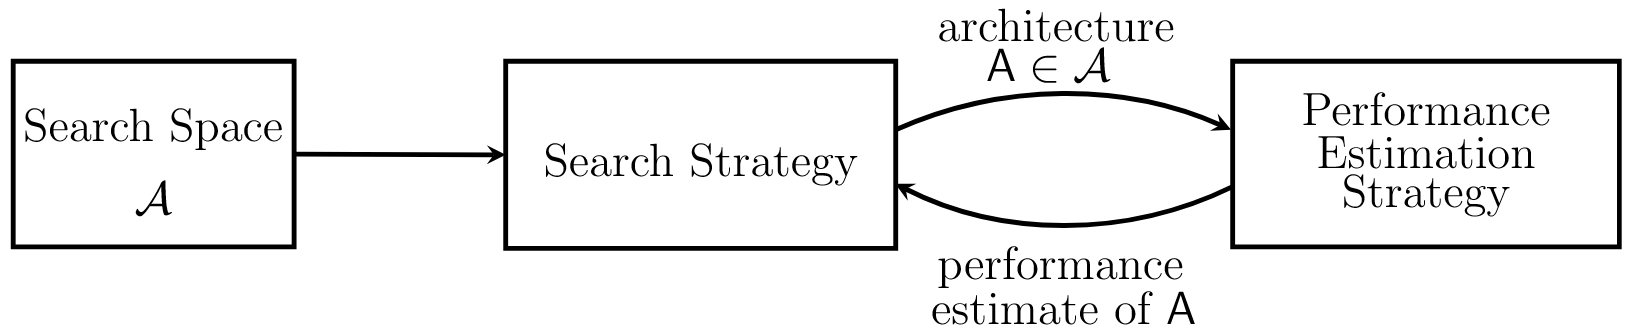
\includegraphics[width=\textwidth,keepaspectratio]{content/chapters/literature_review/discussion/figures/neural_architecture_search_overview.png}
    \captionsource(\acrshort{nas} overview){An abstract overview of the \acrshort{nas} task showing how a search strategy chooses the architecture for a search space and how to preemptively filter architectures that obviously wouldn't be suitable using \acrshort{pes}.\label{fig:neural_architecture_search_overview}}{\citeauthor{elsken_neural_2019}\cite{elsken_neural_2019}}
\end{figure}

Following the layout selection are the actual modules.
Each model has an inventory defined by several neural module types which are dedicated to specific tasks such as finding objects or comparing, etc.
Most of the models discussed have specific, hand-designed module types (S) that are designed to learn best at specific tasks \cite{andreas_deep_2016,hu_learning_2017,hu_explainable_2019,chen_teaching_2022,su_toward_2020,kottur_visual_2018,cho_visual_2021}.
Most models with specific types share a very similar inventory with modules such as finding objects, relocate attention, combine attentions, etc.
Some models implement additional module types for even more specific use-cases such as arithmetic tasks \cite{chen_teaching_2022} or for performing visual coreference resolution \cite{kottur_visual_2018,cho_visual_2021} (see chapters ~\ref{subsec:coreference_neural_module_network} and ~\ref{subsec:neural_module_network_for_visual_dialog}).
There are some models however, which employ an inventory of generic module types referred to as cells (G) that the model must learn itself what modules it should instance and use for solving the tasks for which it's being trained \cite{hudson_compositional_2018,pahuja_learning_2019,chen_meta_2020}.
While the implementations vary across models, they generally posess inputs for at least one or more visual/textual attentions, a general-purpose unit which applies some function/s on the inputs to produce an output, and (optionally) an answering unit for producing the final output that the model will convert to an answer prediction.

Aside from the modules, some models also support a memory structure for storing intermediate mdoule outputs.
In the case of both the \gls{snmn} and \gls{lnmn}, these are in the form of a shared differentiable memory stack.
In both models, the modules/cells are both able to push/pull attention maps to the stack using a soft-selected stack pointer based on the module/cell weights.
The \gls{mac} model also implements memory, but in a different implementation and for a different purpose.
The model is trained with a fixed-length sequence of \gls{mac} cells.
However, each cell has a second output --- besides the attention outputs --- which contains a hidden state created by the previous cell.
The cell can compute a new hidden state for sharing with the next cell but it can also interpolate between this new state and the previous state, effectively deciding whether or not to skip its own reasoning step.
This enables the model to soft-reduce the number of reasoning steps it can use in a differentiable manner.

\subsection{Learning strategies}
\label{subsec:learning_strategies}

Creating a layout and module arrangement is half the problem, the other half is training the model to recognise what works best.
To train the modules and layout generator of a module, a training strategy would need to be employed, either as a single strategy training the model in an end-to-end manner, or multiple strategies working in tandem but training the layout generator and modules separately.

One major factor deciding how the discussed models are trained is their layout differentiability.
If a model constructs its layout using a non-discrete or soft selection (such as the \gls{snmn} model using module weights and text attention), it is considered fully differentiable since the layout selection generated will be unique to the given input and no other input/s.
If the model uses a discrete selection (such as the \gls{n2nmn} model which produces discrete layouts), it is not fully differentiable since different inputs can produce the same non-unique layouts.

As seen in table~\ref{tab:models_module_inventory}, most models are in fact not fully differentiable, using either rule-based parsers\cite{andreas_neural_2016,chen_meta_2020} or \gls{s2s} \gls{rnn}-based layout generators\cite{hu_learning_2017,chen_teaching_2022,su_toward_2020,kottur_visual_2018,cho_visual_2021}.
These models largely use reinforcement learning --- with a layout policy being used to optimise the layout generator --- and using backpropagation on those areas of the model (such as the neural modules) that are differentiable.
On the other hand, the fully-differentiable models all feature a \gls{bilstm} for layout generation and produce variable-length layouts\cite{hudson_compositional_2018}.
These use backpropagation across both the neural modules and layout generator.

Additionally, some models explore different learning beyond just reinforcement or backpropagation.
For instance, \gls{lnmn} uses \gls{darts}\cite{liu_darts_2019} which is a differentiable learning strategy based on backpropagation.
\gls{mmn} --- in contrast to \gls{darts} --- proposed a learning strategy based on the Teacher-Student framework\cite{zimmer_teacher_2014} where a reward/guideline metric is generated by a 'Symbolic Teacher' that the meta modules learn to imitate as `Students'\cite{chen_meta_2020}.

\begin{table}[]
\begin{tabularx}{\linewidth}{cXcXc}
    \toprule
    \multicolumn{5}{c}{VQA/VD Models} \\ \midrule
    Model & \gls{nas} approach & Sel. & Modules & Type  \\
    NMN & Rule-based parsing (see Chapter ~\ref{subsec:neural_module_network}). & D & find, transform, combine, describe, measure & S  \\
    N2NMN & \gls{s2s} \gls{rnn} (See Chapter ~\ref{subsec:n2nmn}). & D & find, relocate, and, or, filter, count, exist, describe, less, more, equal, compare & S  \\
    SNMN & \gls{bilstm}-generated module weights with txt attention (See Chapter ~\ref{subsec:stack_neural_module_network}). & ND & find, transform, and, or, filter, scene, answer, compare, noOp & S  \\
    NMNs\pm{} & Similar to \gls{n2nmn} with type-constrained grammar\cite{gupta_answering_2020}. & D & find, filter, relocate, find-num, find-date, count, compare-num-lt, time-diff, find-max-num, span, compare-date, add, sub & S  \\
    DPNMN & Similar to \gls{n2nmn} with an \gls{rpn} for spatial information. & D & find, relocate, and, or, describe, compare & S  \\
    MAC & \gls{bilstm} and fixed-length cell array where each cell can `skip' itself and relay input to the next cell. & ND & \gls{mac} cells & G  \\
    LNMN & Similar to \gls{snmn} & ND & General modules (Expand further). & G  \\
    MMN & Rule-based parser feeding into a coarse-to-fine program generator. & D & Meta modules & G  \\
    CorefNMN & Similar to \gls{n2nmn} but augmented with a memory network for attention-over-text. & D & find, relocate, and, or, filter, count, exist, describe, less, more, equal, compare, not, refer, exclude & S  \\
    NMNVD & Similar to \gls{corefnmn}. & D & find, relocate, and, refer, describe, compare & S  \\ \bottomrule
\end{tabularx}
\captionsource(Models module inventory)
    {A full breakdown of the model inventory and layout construction architecture of each model discussed. `Selection' denotes whether the module selection of a model is a soft selection (ND) --- and thus trainable with back-propagation --- or fully discrete (D) and instead requires an alternate learning strategy such as reinforcement learning. The `Type' specifies whether the modules listed are `Specified' (S) in that they have a fixed behaviour and only their weights and biases are learned, or they're `Generic' (G) and are able to learn and apply different behaviours without prior implementation or knowledge.\label{tab:models_module_inventory}}
    {Adapted from \citeauthor{fishandi_neural_2023}\cite{fishandi_neural_2023} with additional model information from models covered in this literature review}
\end{table}
